\section{Advanced features of event-driven ABS}
In the previous section we have established the basics of event-driven ABS. It is now clear how events are represented, agent identity is handled, agents receive and schedule events and how they are scheduled and domain-state sampled. Further, by using the \textit{tagless final} approach, we arrived at an elegant, extensible and robust solution, which separates specification - agent and its behaviour - from implementation - the \textit{pure} interpreter. 

In this section we present more advanced concepts of event-driven ABS, necessary in models with much higher complexity than the simple SIR. We developed these concepts using the Sugarscape model as introduced in Chapter \ref{sec:sugarscape}, thus will discuss them from this models perspective. More specifically we show how to create and remove agents dynamically during simulation, add a shared mutable environment, model local mutable agent state and finally how direct agent interactions can be implemented. Together with the basics of event-driven ABS, with these concepts established it should be possible to implement a wide range of event-driven ABS models.

\subsection{Basics of event-driven Sugarscape}
The event-driven approach of Sugarscape alters slightly from the event-driven SIR, discussed before. In the SIR, the dynamics are driven by the pro-activity of the agents through the \textit{MakeContact} and \textit{Recover} events, which the agents (re-)schedule to themselves and thus drive time and the dynamics forward. In Sugarscape, the semantics of the model are different, where in each time-step simply all agents are executed in random order where they perform their actions and interact with each other. Time is advanced discretely, in natural numbers, centrally through the simulation kernel, by scheduling a \textit{Tick} event to each of the agents in random order. Thus, events have no time-stamp associated as there is no need for scheduling of events into the future. Indeed, beside the simulation kernel specific \textit{Tick} event, the model specific events in Sugarscape are used solely for the purpose of agent interactions as will be discussed below. This follows the same approach of the event-driven SIR, where agent interactions between susceptible and infected are implemented by scheduling events with a time-delay of 0. The Sugarscape implementation follows the same idea but does that without the use of time-delays: model specific events are scheduled immediately within the same \textit{Tick} event.

The polymorphic event definition in Sugarscape is thus split into two parts: \textit{Tick}, which is scheduled by the simulation kernel and indicates to the agent the start of a new time-step; \textit{DomainEvent}, which is scheduled by other agents to a specific receiver within a given \textit{Tick} and received by the target agent within the same \textit{Tick}. The \textit{Tick} event carries the time-delta between steps to avoid the necessity of hard-coding it into the agent; \textit{DomainEvent} also carries the sender of the event, to support easy replying to events and avoids the need to add the sender to the actual event type as was done in the event-driven SIR. Due to the discrete time semantics of Sugarscape, where time is advanced in natural numbered steps, time and time-delta between steps are represented both as \textit{Int}.

\begin{HaskellCode}
type Time       = Int
type DTime      = Int
type AgentId    = Int
data ABSEvent e = Tick DTime | DomainEvent AgentId e
\end{HaskellCode}

The fact that Sugarscape schedules event without time-stamps has also implications for the simulation kernel, which does not require a priority queue. The Sugarscape kernel also keeps track of the agents using an \textit{IntMap} for the agent mappings but instead uses a list to keep track of the events. Processing of events is implemented in the pure function \textit{processEvents}, which takes the \textit{EventList}, the simulation state, which contains the agent mappings amongst others, and returns the new simulation state as soon as the event list is empty, indicating that all events in the current \textit{Tick} have been processed.

\begin{HaskellCode}
type EventList e = [(AgentId, ABSEvent e)] -- (receiver, ABSEvent)
processEvents :: RandomGen g => EventList e -> SimulationState g -> SimulationState g
\end{HaskellCode}

The function extracts the event at the front of the \textit{EventList}. In case the list is empty it returns the simulation state unchanged otherwise looks up the receiver and runs it with the given event. Newly scheduled events of the receiver are prepended at the front of the \textit{EventList} through a recursive call. The initial \textit{EventList} passed to \textit{processEvents} is a list with \textit{Tick} events scheduled for every agent, in random order. It is important to understand that the events an agent emits, are prepended to the front of the \textit{EventList}. This ensures that those events are processed next, which is of utmost importance for a correct working of the direct agent interactions discussed below. This also implies that \textit{processEvents} is a potentially non-terminating function, in case there is at least one agent which produces at least one event for every event it receives.

\subsection{Agent-local abstractions}
Some models of ABS in general and Sugarscape in particular require the dynamic creation and removal of agents during simulation. To achieve that, the output type of an agent must be a lot richer than the one in the event-driven SIR. Further, the simulation must provide a mechanism to create new, unique \textit{AgentId} for the newly create agents. Thus, we start with defining a polymorphic agent definition, similar to the event-driven SIR, where the agent takes the \textit{ABSEvent} as input and outputs a tuple of \textit{AgentOut} holding additional information about removal, creation and scheduling of events and a polymorphic output type \textit{o}. The initial Monad stack is a \textit{StateT ABSState}, holding the next agent id and the current simulation time. Using this, the agent can now create new \textit{AgentDef} within its behaviour and return them through the \textit{AgentOut} to the simulation kernel, which can then create a new agent from this definition.

\begin{HaskellCode}
data ABSState = ABSState
  { absNextId :: AgentId -- holds the next agent id 
  , absTime   :: Time    -- current simulation time
  }

type AgentMonad m   = StateT ABSState m
type AgentMSF m e o = MSF (AgentMonad m) (ABSEvent e) (AgentOut m e o, o)

data AgentOut m e o = AgentOut
  { aoKill   :: Any              -- True if this agent should be removed 
  , aoCreate :: [AgentDef m e o] -- a list of agents to create
  , aoEvents :: [(AgentId, e)]   -- a list of events (receiver, event)
  }

data AgentDef m e o = AgentDef
  { adId      :: AgentId         -- unique agent-id
  , adSf      :: AgentMSF m e o  -- the agent behaviour function
  , adInitOut :: o               -- the value of the initial output
  }
\end{HaskellCode}

It is obvious at that point, that scheduling of events in this approach is implemented different than in the event-driven SIR, where the agents Monad stack had a \textit{WriterT} to write events to. The reason for that is that we treat agent-local abstractions different here because of the need to encapsulate local agent state.

TODO: discuss event handler here
TODO: discuss observable agentstate here
TODO: discuss mutable agent state here
TODO: discuss scheduling of events through WriterT here

\subsection{Agent interactions}
TODO: show domainstate events

With the concepts introduced so far we can achieve already a lot in terms of agent-interactions: agents can react to incoming events, which are either the Tick-event advancing simulation time by one step or a message sent by another agent (or the agent itself). This is enough to implement simple one-directional asynchronous agent-interactions where one agent sends a message to another agent but does not await an answer within the same tick. This one-directional asynchronous interactions is used in the model to implement the passing of diseases, the paying back of debt, passing on wealth to children upon death - the agent simply sends a message and forgets about it.

Unfortunately this mechanism is not enough to implement the other agent-interactions in the Sugarscape model, which are structurally richer: they need to be synchronous. In the use-cases of mating, trading and lending two agents need to come to an agreement over multiple interactions steps within the same tick which need to be exclusive and synchronous.  This means that an agent A initiates such a multi-step conversation with another agent B by sending an initial message to which agent B has to react by a reply to agent A who upon reception of the message, will pick up computation from that point and reply with a new message and so on. Both agents must not interact with other agents during this conversation to guarantee resource constraints, otherwise it would become quite difficult and cumbersome to ensure that agents don't spend more than they have when trading with multiple other agents at the same time. Also the initiating agent A must be able to pick up processing of its Tick event from the point where it started the conversation with agent B because sending a message always requires the handling of the current event to exit and hand the control back to the simulation kernel. See Figure \ref{fig:syncagentinteractions} for a visualisation of the sequence of actions.

\begin{figure}
	\centering
	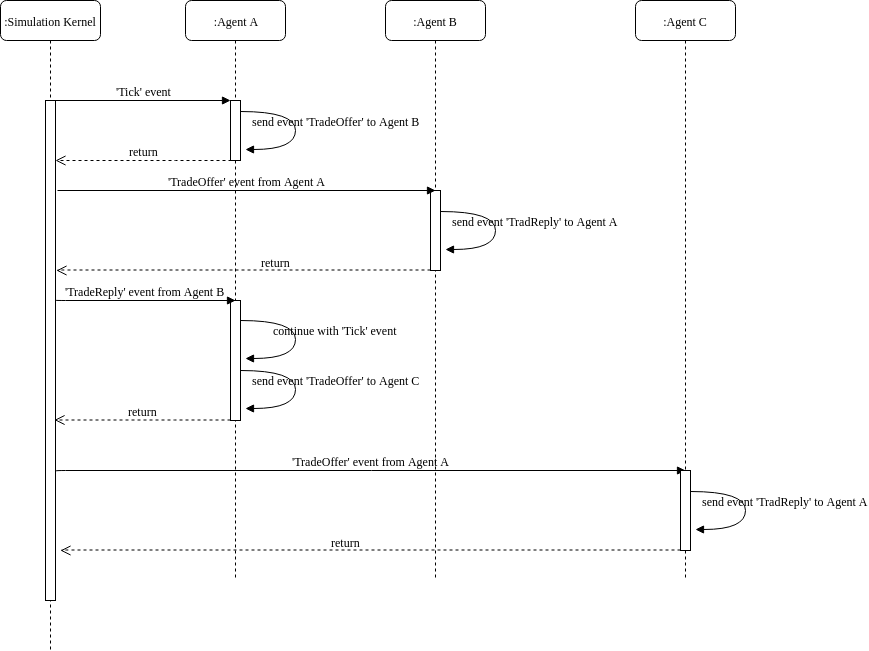
\includegraphics[width=1.0\textwidth, angle=0]{./fig/eventdriven/syncagentinteractions.png}
	\caption{Sequence diagram of synchronous agent-interaction with the trading use-case. Upon the handling of the 'Tick' event, Agent A looks for trading partners and finds Agent B within its neighbourhood and sends a 'TradingOffer' message. Agent B replies to this message and Agent A continues with the trading algorithm by picking up where it has left the execution when sending the message to Agent B. After Agent A has finished the trading with Agent B, it turns to Agent C, where the same procedure follows and is thus not included fully in this diagram.}
	\label{fig:syncagentinteractions}
\end{figure}

The way to implement this is to allow an agent to be able to change its internal event-handling state: to switch into different event-handlers, after having sent an event, to be able to react to the incoming reply in a specific way by encapsulating local state for the current synchronous interaction through closures and currying. Further by making use of continuations the agent can pick up the processing of the 'Tick' event after the synchronous agent-interaction has finished. Key to this is the function \textit{continueWithAfter} which we already shortly introduced through \textit{generalEventHandler}. This function takes an MSF which returns an output b and an optional MSF. If this optional Maybe MSF is Just then the \textit{next} input is handled by this new MSF. In case no new MSF is returned (Nothing), the MSF will stay the same. This is a more specialised version of the \textit{switch} combinator introduced in Chapter \ref{sec:back_frp} in the way that it doesn't need an additional function to produce the actual MSF continuation. Note that the semantics are different though: whereas \textit{continueWithAfter} only applies the new MSF in the \textit{next} step, \textit{switch} runs the new MSF immediately. The implementation of the function is as follows:

\begin{HaskellCode}
continueWithAfter :: Monad m => MSF m a (b, Maybe (MSF m a b)) -> MSF m a b
continueWithAfter msf = MSF (\a -> do
  ((b, msfCont), msf') <- unMSF msf a
  let msfNext = fromMaybe (continueWithAfter msf') msfCont
  return (b, msfNext))
\end{HaskellCode}

We can now look at the Tick handling function. It returns a Maybe (EventHandler g) which if is Just will result in to a change of the top-level event handler through \textit{continueWithAfter} as shown in \textit{generalEventHandler} above. Note the use of continuations in the case of \textit{agentMating, agentTrade, agentLoan}. All these functions return a Maybe (EventHandler g) because all of them can potentially result in synchronous agent-interactions which require to change the top-level event handler. When calling \textit{agentDisease} we are passing a default continuation which simply switches back into \textit{generalEventHandler} to finish the processing of a Tick in an agent.

\begin{HaskellCode}
handleTick :: RandomGen g => DTime -> AgentLocalMonad g (Maybe (EventHandler g))
handleTick dt = do
  agentAgeing dt
  
  harvestAmount <- agentMove
  metabAmount   <- agentMetabolism
  agentPolute harvestAmount metabAmount

  ifThenElseM
    (starvedToDeath `orM` dieOfAge)
    (do
      agentDies agentMsf
      return Nothing) 
    -- pass agentContAfterMating as continuation to pick up after mating
    -- synchronous conversations have finished
    (agentMating agentMsf agentContAfterMating)

-- after mating continue with cultural process and trading
agentContAfterMating :: RandomGen g => AgentLocalMonad g (Maybe (EventHandler g))
agentContAfterMating = do
    agentCultureProcess
    -- pass agentContAfterTrading as continuation to pick up after trading 
    -- synchronous conversations have finished
    agentTrade agentContAfterTrading 

-- after trading continue with lending and borrowing
agentContAfterTrading :: RandomGen g  => AgentLocalMonad g (Maybe (EventHandler g))
agentContAfterTrading = agentLoan agentContAfterLoan

-- after lending continue with diseases, which is the step in a Tick event
agentContAfterLoan :: RandomGen g => AgentLocalMonad g (Maybe (EventHandler g))
agentContAfterLoan = agentDisease defaultCont

-- safter diseases imply switch back into the general event handler
defaultCont :: RandomGen g => AgentLocalMonad g (Maybe (EventHandler g))
defaultCont = return (Just generalEventHandler)
\end{HaskellCode}

\subsubsection{Synchronous through Tagless Final}
TODO: the indirect, continuation based approach is cumbersome and it is easy to get something wrong, thus synchronous interactions would be desirable. With the tagless final approach as introduced in the TODO section, this becomes possible
TODO: show the syncSend approach of SIR and discuss the problem of not being able to recursively send to itself e.g. agent A initiates syncSend, then it cannot send directly to itself or if it sends to agent B this agent B cannot send another syncSend to agent A. Or A -> B -> C -> A is also not possible, any chain which comes back to the originator leads to wrong semantics where effects might be visible but the changes to the last agent will be overridden.

\subsection{Shared mutable environment}
TODO 

Environment representation is quite simple, after we have solved the problem of how the agent can access it by using StateT. It is only a matter of selecting the right data-structure and writing domain-specific functions of the corresponding model to mutate the environment. Initially we used an indexed array from the \textit{array} package. This data-structure has excellent read performance but in performance tests it was shown that it has serious performance and memory leak issues with updates, leading to allocation of about 40 MByte / second on our machine. Clearly this is unacceptable for simulation purposes, which often requires software to run for hours, and thus needs a constant memory consumption and must prevent even slowly linearly increasing memory usage under all costs. The solution was to switch to \textit{IntMap} from the \textit{containers} package as an underlying data-structure. We used the discrete 2d-coordinates to map the environment cells to a unique index. This solved both the performance and memory leak issues completely.

We must make a clear distinction between the environments data-structure and how agents access it and the environments behaviour. In the Sugarscape model, the behaviour of the environment is quite trivial: it simply regrows resources over time and diffuses pollution in case pollution is turned on. This behaviour is achieved by providing a pure function without any monadic context or MSF. This is not necessary because the environment how we implement it, does not encapsulate local state and it does not interact with agents through messages and vice versa. Thus a pure function which maps the environment to the environment is enough: \textit{Time $\rightarrow$ SugEnvironment $\rightarrow$ SugEnvironment}. Further it also takes the current simulation time so it can implement seasons, where the speed of regrowth of resources is different in different regions and swaps after some time. This function is called in the simulation kernel after every Tick (see below).

Generally, one can distinguish between four different types of environments in ABS:

\begin{enumerate}
	\item \textit{Passive read-only} - implemented in Chapter \ref{sec:timedriven_firststep}, where the environment itself is not modelled as an active process and is static information, e.g. a list of neighbours, passed to each agent. The agents cannot change the environment actively - in the case of Chapter \ref{sec:timedriven_firststep} this is enforced at compile time by simply excluding it from the data an agent can emit. Note the agents change the environment implicitly by changing their state but there is no notion of an active environment process.
	
	\item \textit{Passive read/write} - implemented in Chapter \ref{sec:adding_env}. The environment is just shared data, which can be accessed and manipulated by the agents. Note that this forces some arbitration mechanism to prevent conflicting updates e.g. running the agents sequentially one after the other, to ensure that only one agent has access at a time.
	
	\item \textit{Active read/write} - as implemented above. To make it active a pure function is used where the environment data is owned by the simulation kernel and then made available to the agents through a State Monad. Another approach would be to implement the environment process as an agent, which is run together with all the other agents. This allows the environment to send and receive messages but the guarantees about when the environment will be run is lost if agents are run random sequentially.
	
	\item \textit{Active read-only} - can be implemented as above but instead of providing the environment data through a State Monad, a Reader Monad is used. The environment data is owned by the Simulation kernel and the process runs as a pure function as before but the data is provided in a read-only way through the Reader Monad.
\end{enumerate}